\documentclass[10pt, UKenglish]{beamer}
\usepackage{babel}
\usepackage[utf8]{inputenc}  
\usepackage{geometry}
\usepackage[customcolors]{hf-tikz}
\usepackage[T1]{fontenc}   
\usepackage{tcolorbox}
\usepackage{siunitx}
\usepackage{hyperref}
\usepackage{bookmark}
\usepackage{marvosym}
\usepackage{tikz}
\usepackage{tikz-qtree}
\usepackage{cancel}
\usepackage{todonotes}
\useoutertheme[subsection=false]{smoothbars}
\DeclareSIUnit[number-unit-product = {}]{\inchQ}{\textquotedbl}
\usepackage{amsmath}
\usepackage{amssymb}
\newcommand\hmmax{0} % default 3
% \newcommand\bmmax{0} % default 4
\usepackage{bm} 
\DeclareSIUnit[number-unit-product = {\thinspace}]{\inch}{in}
\usetheme[menuwidth={0.3\paperwidth}]{erlangen}
\usepackage{multicol}
\usepackage{charter}
\setbeamercovered{transparent=20}
\setbeamertemplate{navigation symbols}{}
\sisetup{separate-uncertainty = true}
\usepackage[version=4]{mhchem}
\usepackage{tikz}
\usepackage{hepnames}
\usepackage{soul}
\usepackage{color}
\usepackage{thesis_defs}
\usepackage{subcaption}
\usepackage{xcolor}
\usepackage{enumitem}
\setlist[enumerate]{labelindent=10pt,style=multiline,leftmargin=2.5cm}
\setlist[itemize]{font=$\bullet$\scshape\bfseries}

\usepackage[backend=biber]{biblatex}
\bibliography{bibliography.bib}

\graphicspath{%
  {../../feynman_diagrams/}%
  {../feature_plots/}%
  {./figures_theory/}%
  {./figures_simple/}%
  {./figures_misc/}%
  {./app1/}%
  {./app2/}%
  {./app3/}%
}


\definecolor{color1}{RGB}{33,217,217}
\definecolor{color2}{RGB}{7,61,111}

\newcommand{\lr}{\mathcal{lr}}


\newcounter{totavalue}
\newcounter{parvalue}

\def\aux{1}
\def\radius{9pt}
\def\step{4pt}
\usepackage[absolute,overlay]{textpos}


\newcommand\circcounter{%
\ifnum\inserttotalframenumber<2\relax
\else
  \setcounter{totavalue}{\inserttotalframenumber}
  \setcounter{parvalue}{\insertframenumber}
  \ifnum\inserttotalframenumber>45\relax
    \renewcommand\step{0pt}
  \fi%
  \pgfmathsetmacro{\aux}{360/11}
  \begin{tikzpicture}[remember picture,overlay, rotate=90+\aux]
  \foreach \i in {0,1,...,11}
    \fill[logo_blue] 
      (0,0) -- (-\i*\aux:\radius) arc  (-\i*\aux:-(\i+1)*\aux+\step:\radius) -- cycle;
  \foreach \i in {1,...,\insertframenumber}
    \fill[logo_grey] 
      (0,0) -- (-\i*\aux:\radius) arc  (-\i*\aux:-(\i+1)*\aux+\step:\radius) -- cycle;
  \fill[white] circle (\radius/1.3);
  \node at (0,0) {\small\insertframenumber}; 
  \end{tikzpicture}%
\fi%
}


\usepackage{eso-pic,picture}



\begin{document} 

\title[Bachelorvortrag]{Hadhad MVA}
\subtitle{21st of September 2021}
\author{Christian Kirfel}
%\institute{Universtität Bonn}
        



\begin{frame}[plain]
\vspace{0.0cm}
  \titlepage
      \AddToShipoutPictureFG*{%
    \AtPageUpperLeft{%
      \put(8.7cm,-9.6cm){

\includegraphics[scale=0.03]{original_logo.jpg}
\makebox(0,0)[lt]{}%
      }%
    }%
  }%
    \AddToShipoutPictureFG*{%
    \AtPageUpperLeft{%
      \put(0.0cm,-9.6cm){
%\includegraphics[scale=0.17]{atlas_gay.png}

\includegraphics[scale=0.17]{ATLAS-Logo-Ref-RGB-H_0.jpg}
\makebox(0,0)[lt]{}%
      }%
    }%
  }%
\end{frame}
\addtobeamertemplate{navigation symbols}{\vspace*{0.8cm}\hfill\circcounter\hspace*{0.7cm}}




\begin{frame}{Event selection}
    \begin{columns}
      \begin{column}{0.5\textwidth}
        \centering 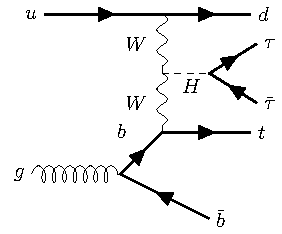
\includegraphics[width=0.8\textwidth]{/cephfs/user/s6chkirf/feynman_diagrams/tHq_tautau}\\
                \begin{itemize}
          \item n-jets: at least 2 (b-jets: \textbf{>0})
          \item b-jet WP: 70 DL1r
          \item nLeptons \& nTaus: $\bf{1e / \mu~2\tau_{\text{had}}} $
          \item $E_{\text{T,miss}}$: no cut (to \SI{800}{GeV})
        \end{itemize}
      \end{column}
      \begin{column}{0.7\textwidth}
        \vspace*{-0.05\textwidth}
        \begin{itemize}
          \footnotesize
          \item jets:
          \vspace*{-0.02\textwidth}
          \begin{itemize}
            \footnotesize
            \item $p_T>\SI{35}{GeV}$
            \item $|\eta|<4.5$
            \item EMPFlow
          \end{itemize}
          \item electrons:
          \vspace*{-0.02\textwidth}
          \begin{itemize}
            \footnotesize
            \item $p_T>\SI{20}{GeV}$ leading \SI{27}{GeV}
            \item $|\eta|<2.5$ not in 1.37 - 1.52
            \item WP: LooseAndBLayerLH ; \\isolation: no requirement
          \end{itemize}
          \item muons:
          \vspace*{-0.02\textwidth}
          \begin{itemize}
            \footnotesize
            \item $p_T>\SI{20}{GeV}$ leading \SI{27}{GeV}
            \item $0.01<|\eta|<2.5$
            \item WP: Loose ; isolation: no requirement
          \end{itemize}
          \item taus:
          \vspace*{-0.02\textwidth}
          \begin{itemize}
            \footnotesize
            \item $p_T>\SI{20}{GeV}$ leading \SI{27}{GeV}
            \item $|\eta|<2.5$ not in 1.37 - 1.52
            \item WP: RNNLoose
            \item ASG recommended OLR ($\tau_{had}$ remove jets)
          \end{itemize}
        \end{itemize}
      \end{column}
    \end{columns}
\end{frame}
%
\begin{frame}{Data/MC agreement}
  \centering 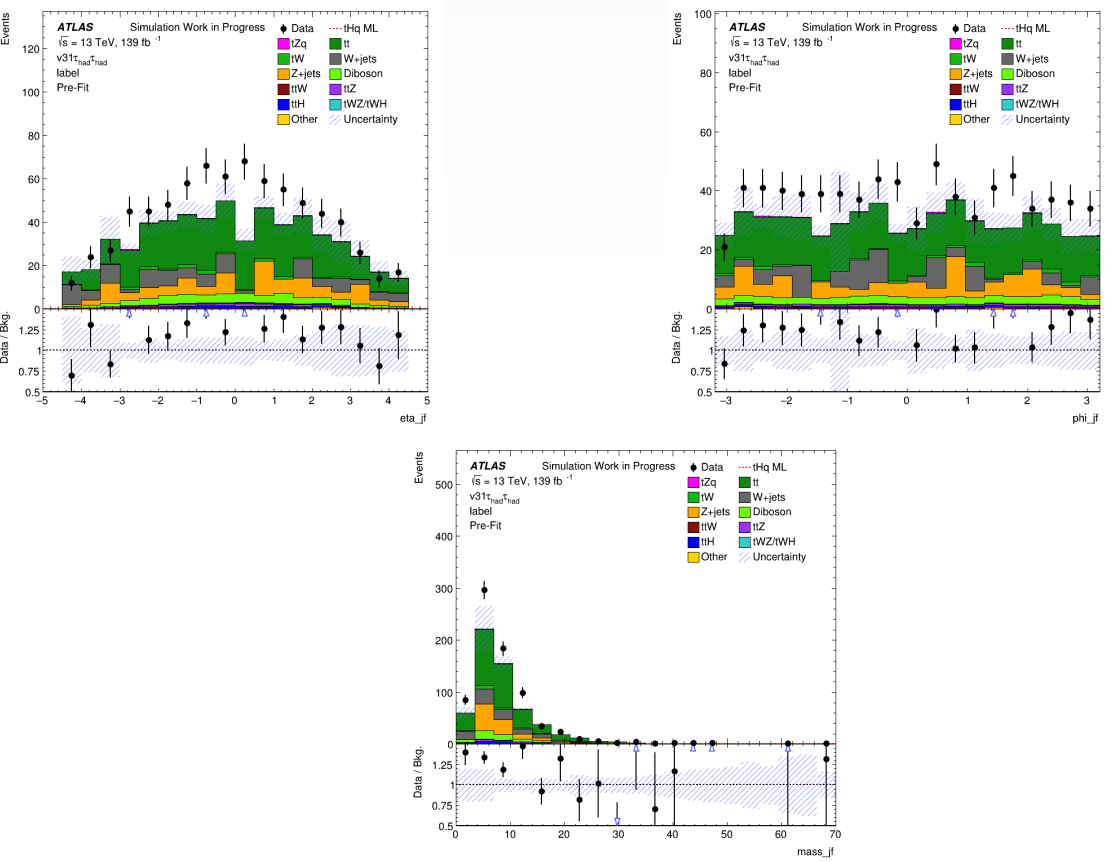
\includegraphics[width=0.9\textwidth]{data_mc_agreement}
\end{frame}
%
\begin{frame}{Correlation}
  plots to be added
\end{frame}
%
\begin{frame}{Preliminary feature selection}
  \centering Mostly final state kinematics
    \begin{columns}
        \begin{column}{0.5\textwidth}
            \resizebox{\linewidth}{!}{
            \begin{tabular}{|l|l|}
                \hline
                eta\_jf              & forward jet eta                        \\ \hline
                pt\_jf               & forward jet transverse momentum        \\ \hline
                mass\_jf             & forward jet mass                       \\ \hline
                phi\_jf              & forward jet phi                        \\ \hline
                eta\_b               & b-jet eta                              \\ \hline
                pt\_b                & b-jet transverse momentum              \\ \hline
                phi\_b               & b-jet phi                              \\ \hline
                mass\_b              & b-jet mass                             \\ \hline
                m\_met               & Missing energy                         \\ \hline
                Reco\_w\_mass\_2     & Reconstructed mass of the W case 1     \\ \hline
                Reco\_w\_mass\_1     & Reconstructed mass of the W case 2     \\ \hline
                fs\_had\_tau\_1\_pt  & Hadronic tau 1 pt                      \\ \hline
                fs\_had\_tau\_1\_eta & Hadronic tau 1 eta                     \\ \hline
                fs\_had\_tau\_2\_pt  & Hadronic tau 2 pt                      \\ \hline
                fs\_had\_tau\_2\_eta & Hadronic tau 2 eta                     \\ \hline
            \end{tabular}}
        \end{column}
        \begin{column}{0.5\textwidth}
            \resizebox{\linewidth}{!}{
            \begin{tabular}{|l|l|}
                 \hline
                 deltaRTau        & Delta R of the hadronic taus          \\ \hline
                 deltaPhiTau      & Delta phi of the hadronic taus        \\ \hline
                 HvisMass         & mass of LorentzV sum of hadronic taus  \\ \hline
                 HvisPt           & pt of LorentzV sum of hadronic taus      \\ \hline
                 HvisEta          & eta of LorentzV sum of hadronic taus      \\ \hline
                 TvisMass         & mass of reconstructed top             \\ \hline
                 TvisPt           & pt of visible top                     \\ \hline
                 TvisEta          & eta of visible top                    \\ \hline
                 M\_b\_jf         & Mass of LorentV sum of b and jf       \\ \hline
                 HT               & Sum of transverse energies            \\ \hline
                 lep\_Top\_pt     & Light lepton pt                       \\ \hline
                 lep\_Top\_eta    & Light lepton eta                      \\ \hline
             \end{tabular}}
        \end{column}
    \end{columns}
\end{frame}
%
\begin{frame}{Feature ranking}
  WIP
\end{frame}
%
\begin{frame}{Negative weight handling}
  \begin{columns}
    \begin{column}{0.5\textwidth}
      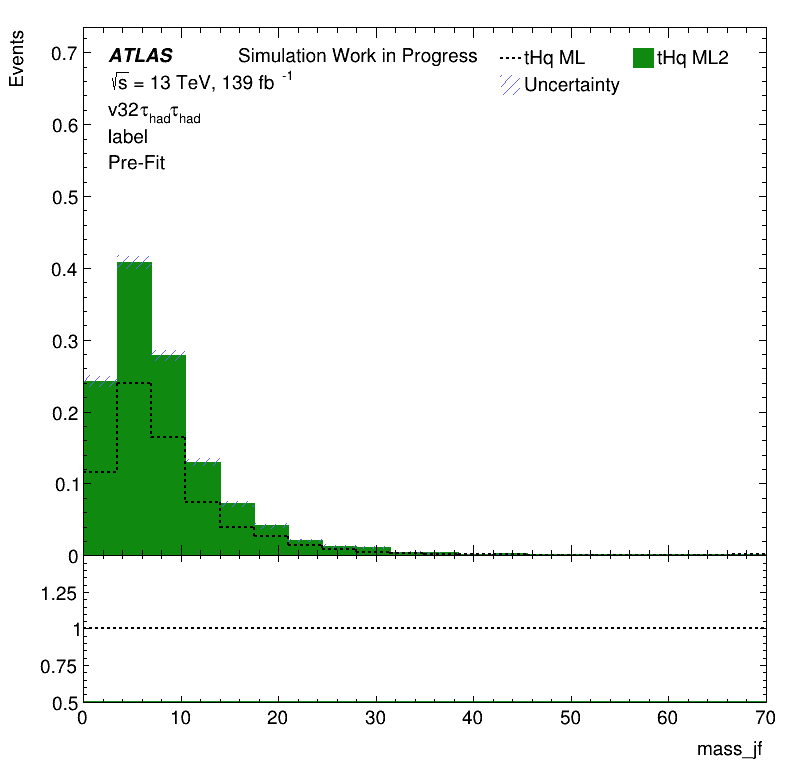
\includegraphics[width=0.7\textwidth]{mass_jf}
      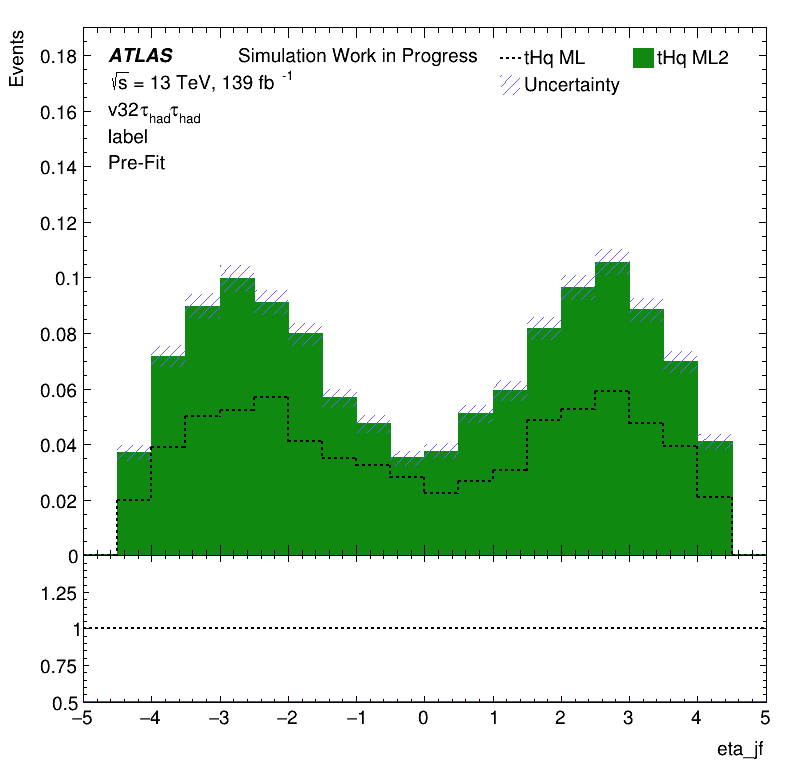
\includegraphics[width=0.7\textwidth]{eta_jf}
    \end{column}
  %
    \begin{column}{0.5\textwidth}
      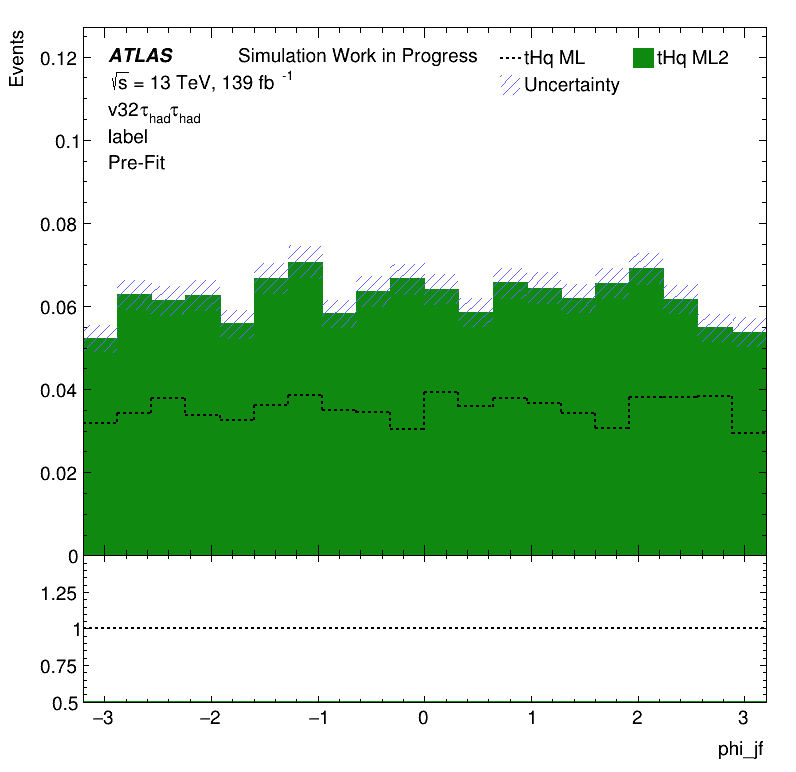
\includegraphics[width=0.7\textwidth]{phi_jf}
      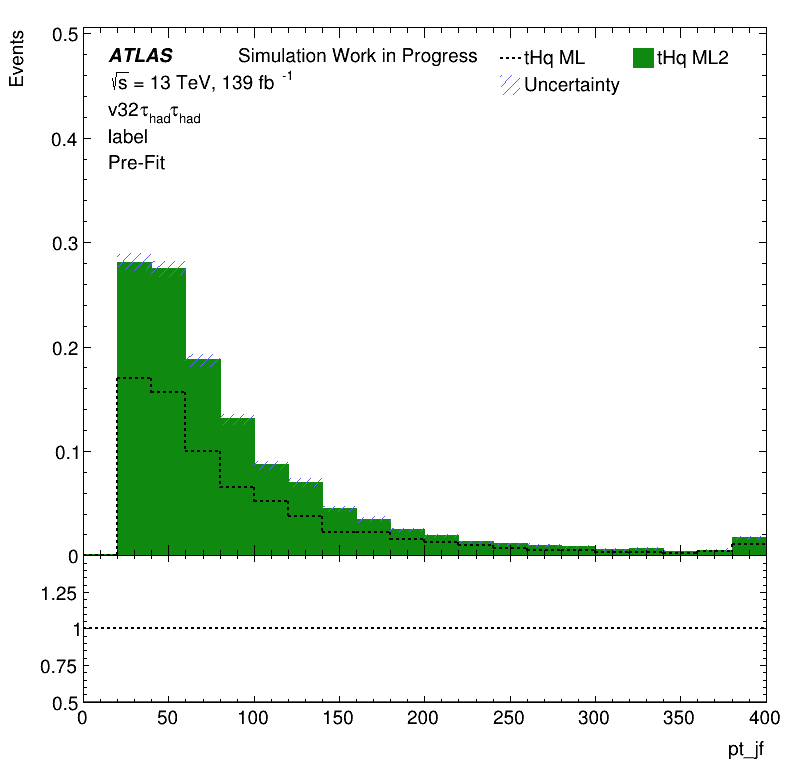
\includegraphics[width=0.7\textwidth]{pt_jf}
    \end{column}
  \end{columns}
\end{frame}
%
\begin{frame}{Negative weight correlation}
  \centering 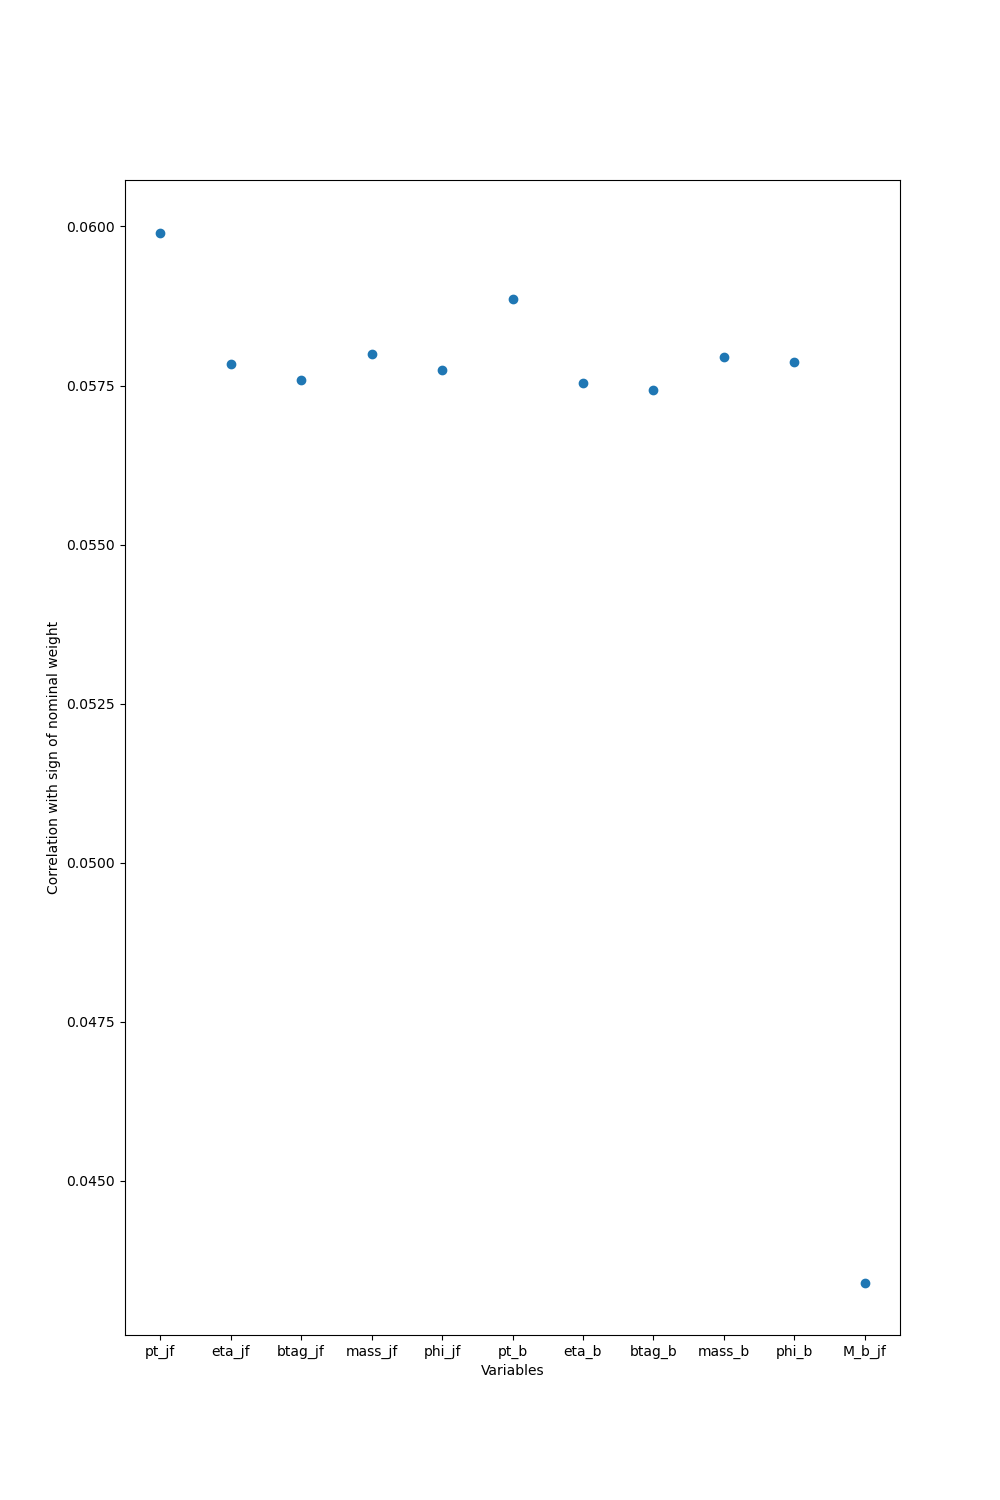
\includegraphics[width=0.5\textwidth]{negWeight_sign_corr}
\end{frame}
%
\begin{frame}{Input preparation}
  WIP
\end{frame}
%
\begin{frame}{Network Hyperparamterts}
  \begin{itemize}
    \item Coarse optimisation: Evolutionary
    \item Fine optimisation: Grid search
  \end{itemize}
    \begin{table}[]
    \begin{tabular}{|l|l|}
    \hline
    Hyperparameter          &     Setting              \\ \hline
    Model                   &     Categorical          \\ \hline
    Nodes                   &     120                  \\ \hline
    Layers                  &     6                    \\ \hline
    Dropout                 &     0.65                 \\ \hline
    Batchnormalisation      &     On                   \\ \hline
    Activation              &     elu                  \\ \hline
    Output activation       &     softmax              \\ \hline
    Batch size              &     1000                 \\ \hline
    Optimisation            &     Adam                 \\ \hline
    Weight Initialisation   &     Lecun Normalisation  \\ \hline
    K-folds                 &     4                    \\ \hline
    \end{tabular}
    \end{table}
\end{frame}
%
\begin{frame}{Results}
      \begin{columns}
        \begin{column}{0.5\textwidth}
          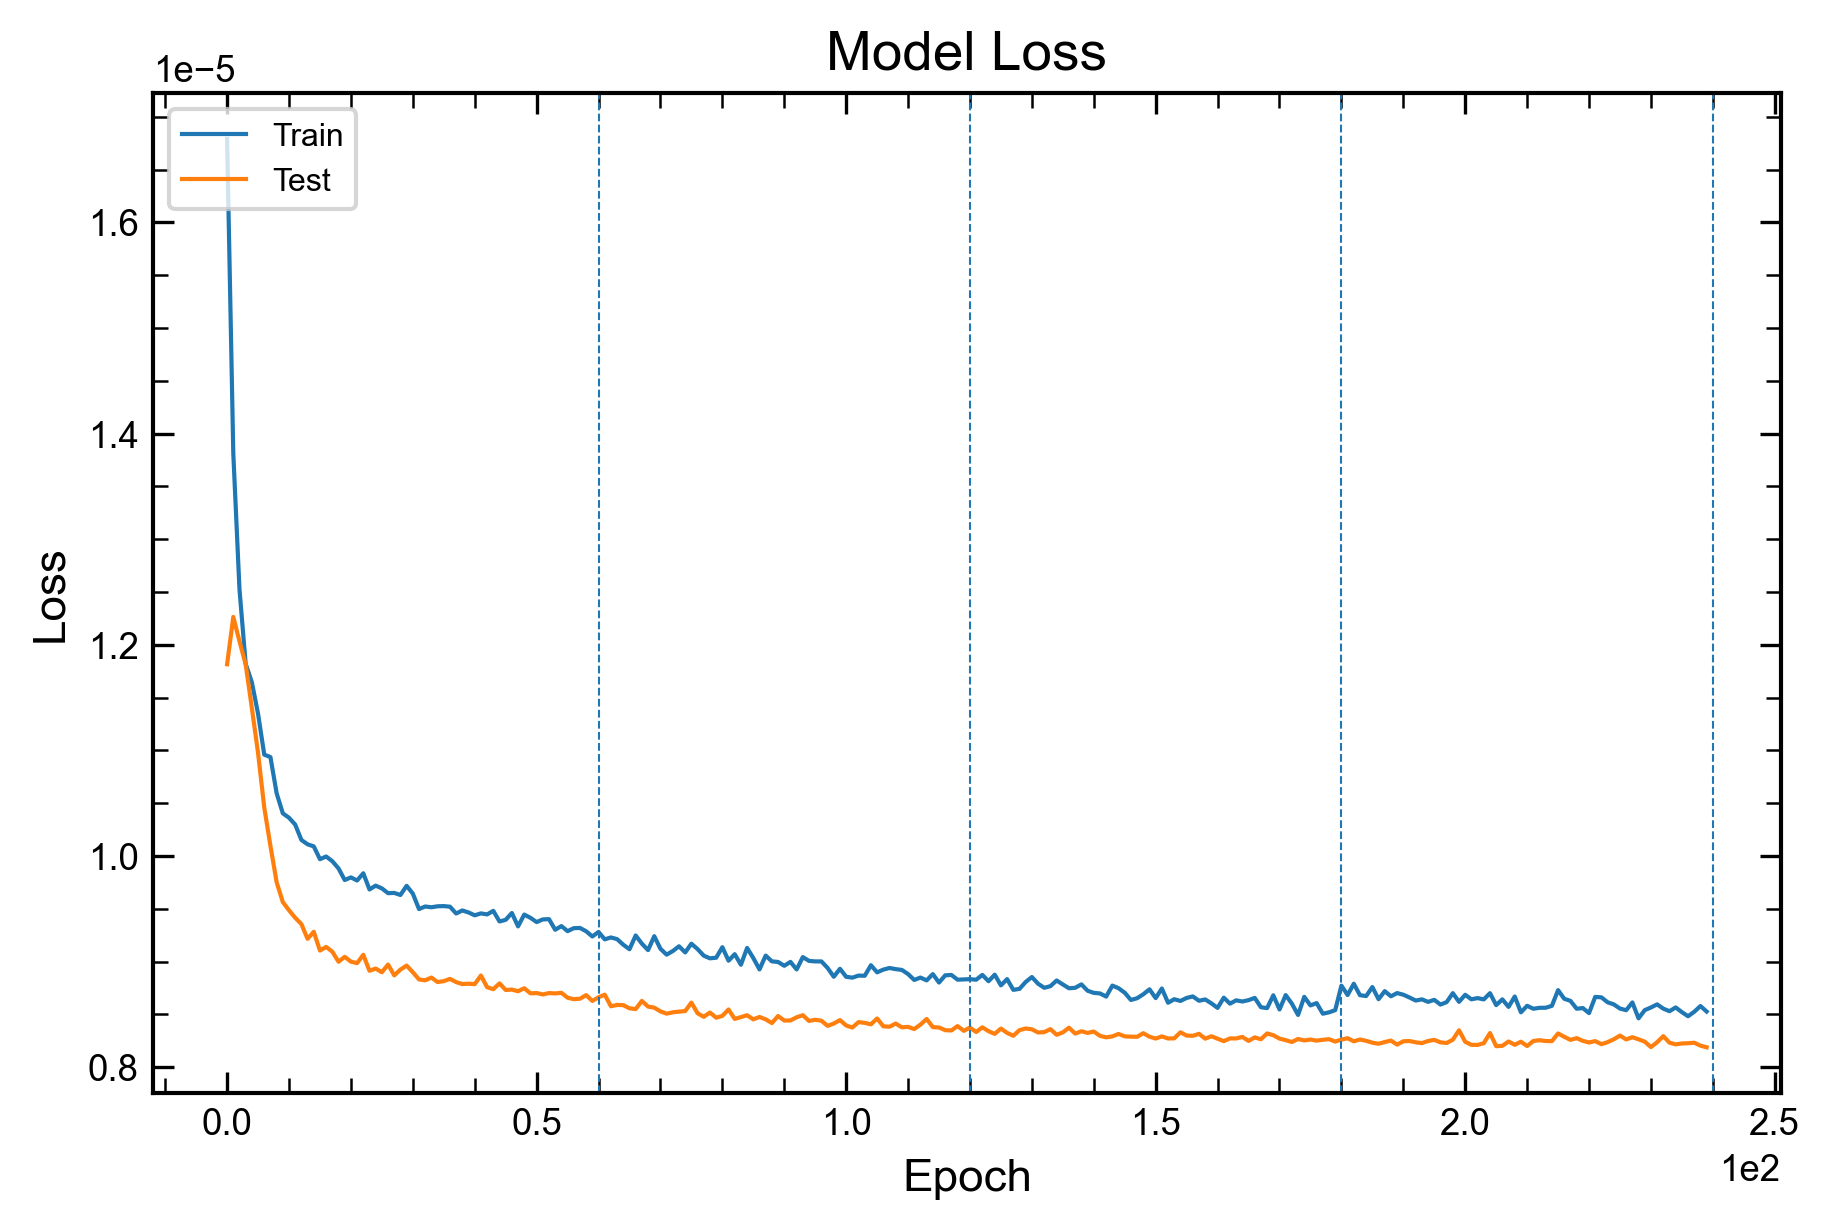
\includegraphics[width=0.8\textwidth]{losses_cat}
          \begin{itemize}
            \item Stable training
            \item Good AUC
          \end{itemize}
        \end{column}
        \begin{column}{0.5\textwidth}
          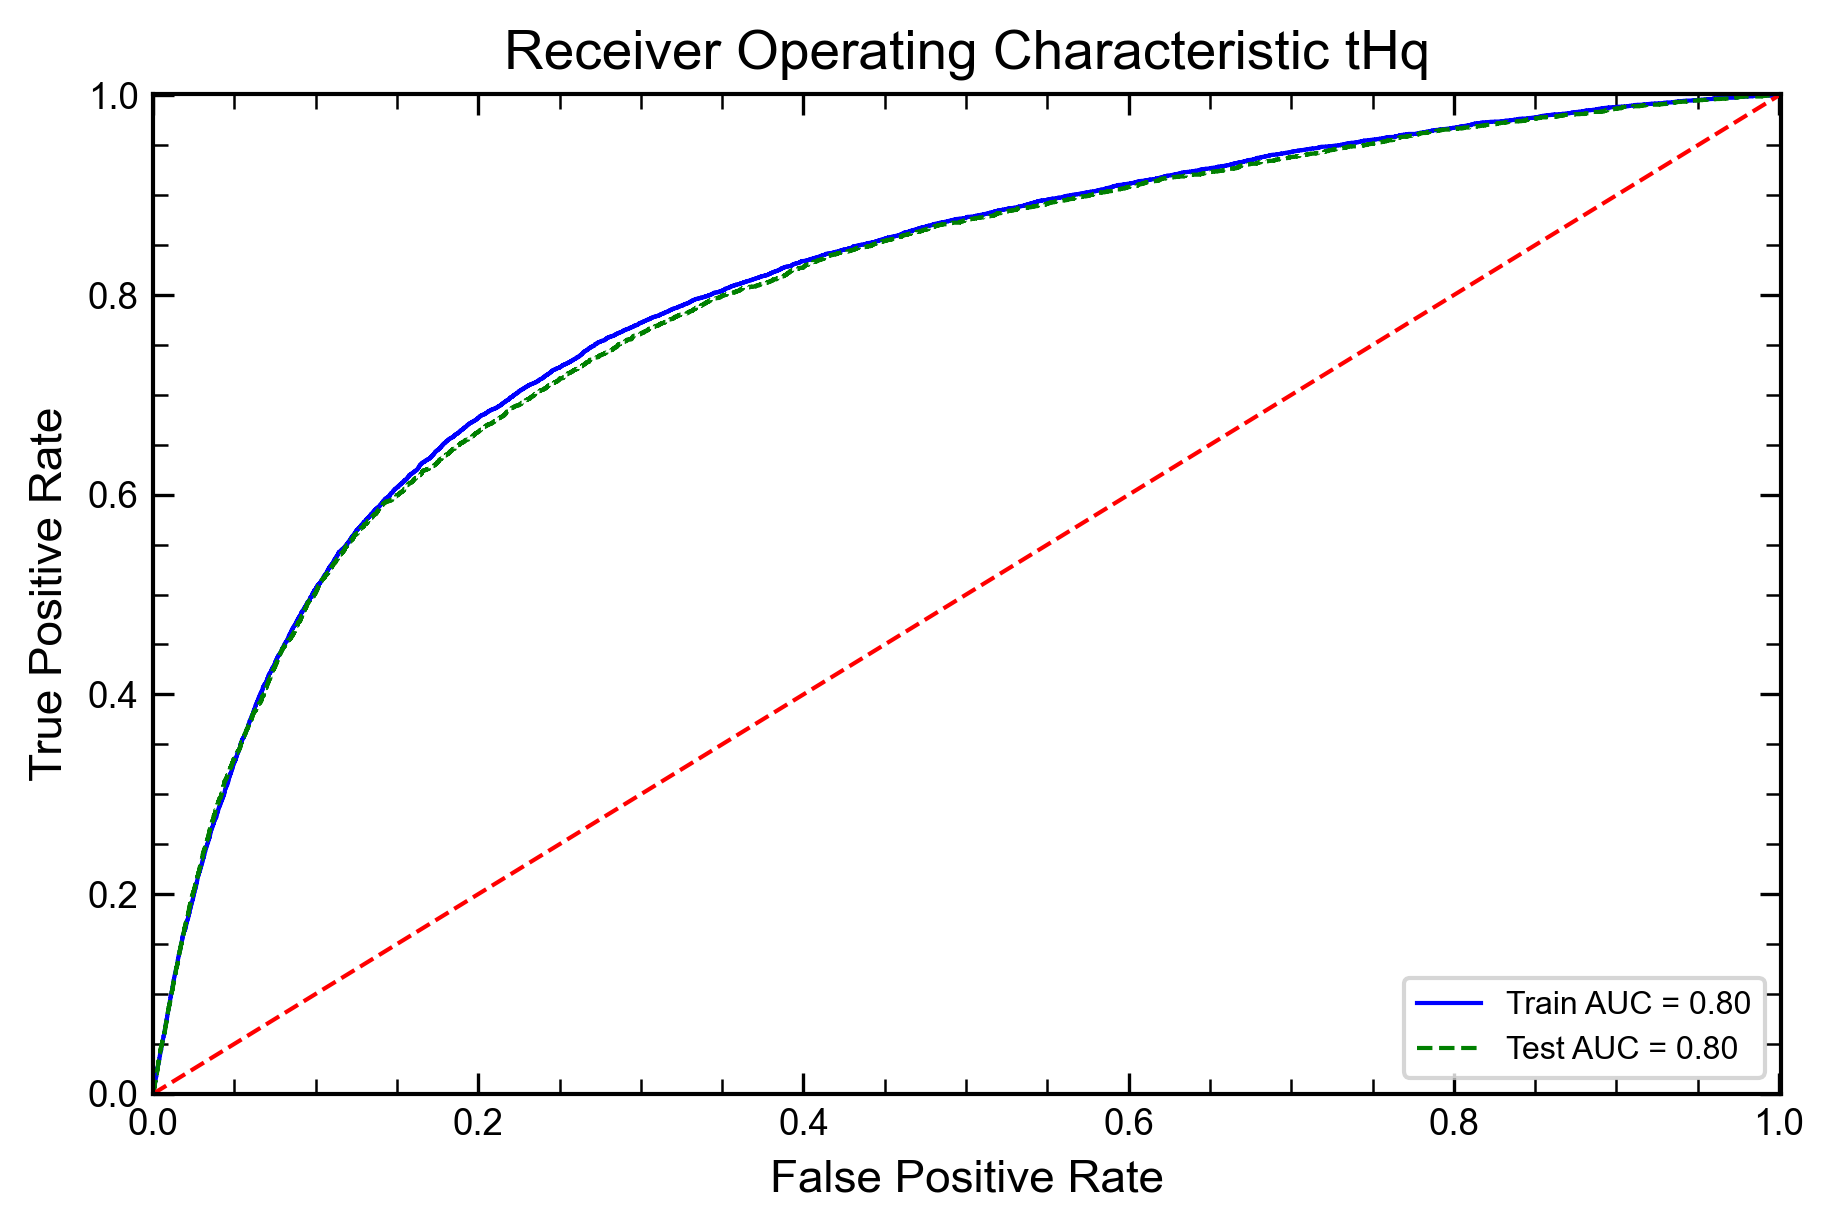
\includegraphics[width=0.8\textwidth]{ROC_cat}
          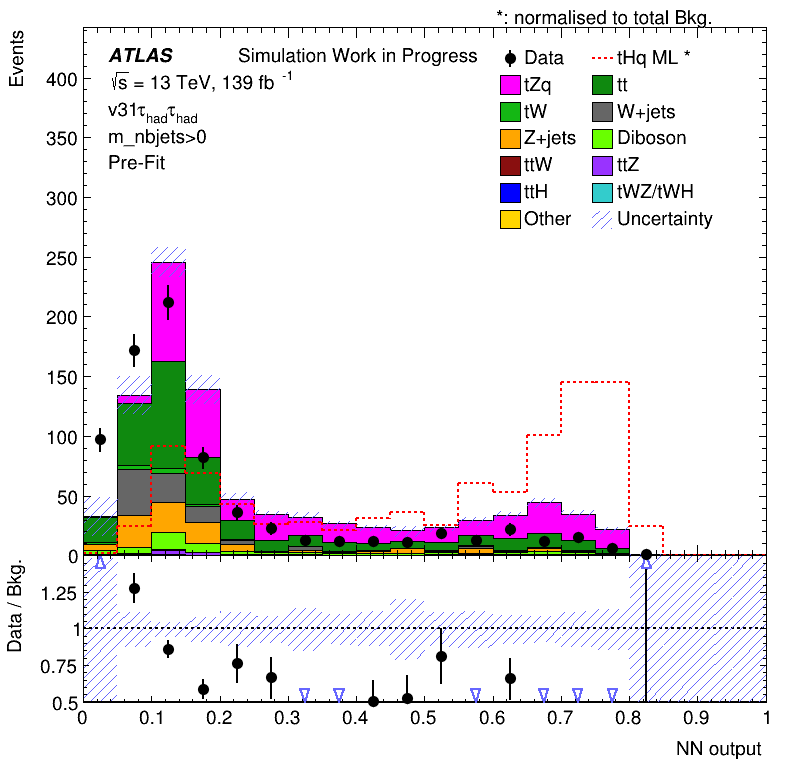
\includegraphics[width=0.8\textwidth]{response_cat}
        \end{column}
    \end{columns}    
\end{frame}


%
%

  

\end{document}